% !Mode:: "TeX:UTF-8"
%
% 第五章：实验
%
% 本节展示的用法：
%   - 结果表格（三线表 + 加粗突出）
%   - 图片插入
%   - 交叉引用（\ref{} 引用图表）
%   - 段落文字
%

\chapter{实验评估与结果分析}
\echapter{Experimental Evaluation and Analysis}
\label{chap:experiments}

本章通过实验评估所提方法的有效性。

\section{实验设置}
\esection{Experimental Setup}
\label{sec:setup}

实验环境配置：Intel i7-12700K，NVIDIA RTX 3090，PyTorch 2.0。评价指标包括准确率（Accuracy）和 F1 分数。

\section{主要结果}
\esection{Main Results}
\label{sec:main_results}

表\ref{tab:results}展示了与基线方法的对比结果。

\begin{table}[htbp]
\centering
\caption{与基线方法的性能对比}
\label{tab:results}
\begin{tabular}{lccc}
\toprule
方法 & 准确率 (\%) & F1 分数 & 训练时间 (min) \\
\midrule
基线 A & 85.32 & 0.842 & 45 \\
基线 B & 87.15 & 0.861 & 52 \\
\textbf{本文方法} & \textbf{91.27} & \textbf{0.905} & 50 \\
\bottomrule
\end{tabular}
\end{table}

\section{收敛性分析}
\esection{Convergence Analysis}
\label{sec:convergence}

图\ref{fig:convergence}展示了训练过程中的损失曲线，模型能够快速稳定收敛。

\begin{figure}[htbp]
\centering
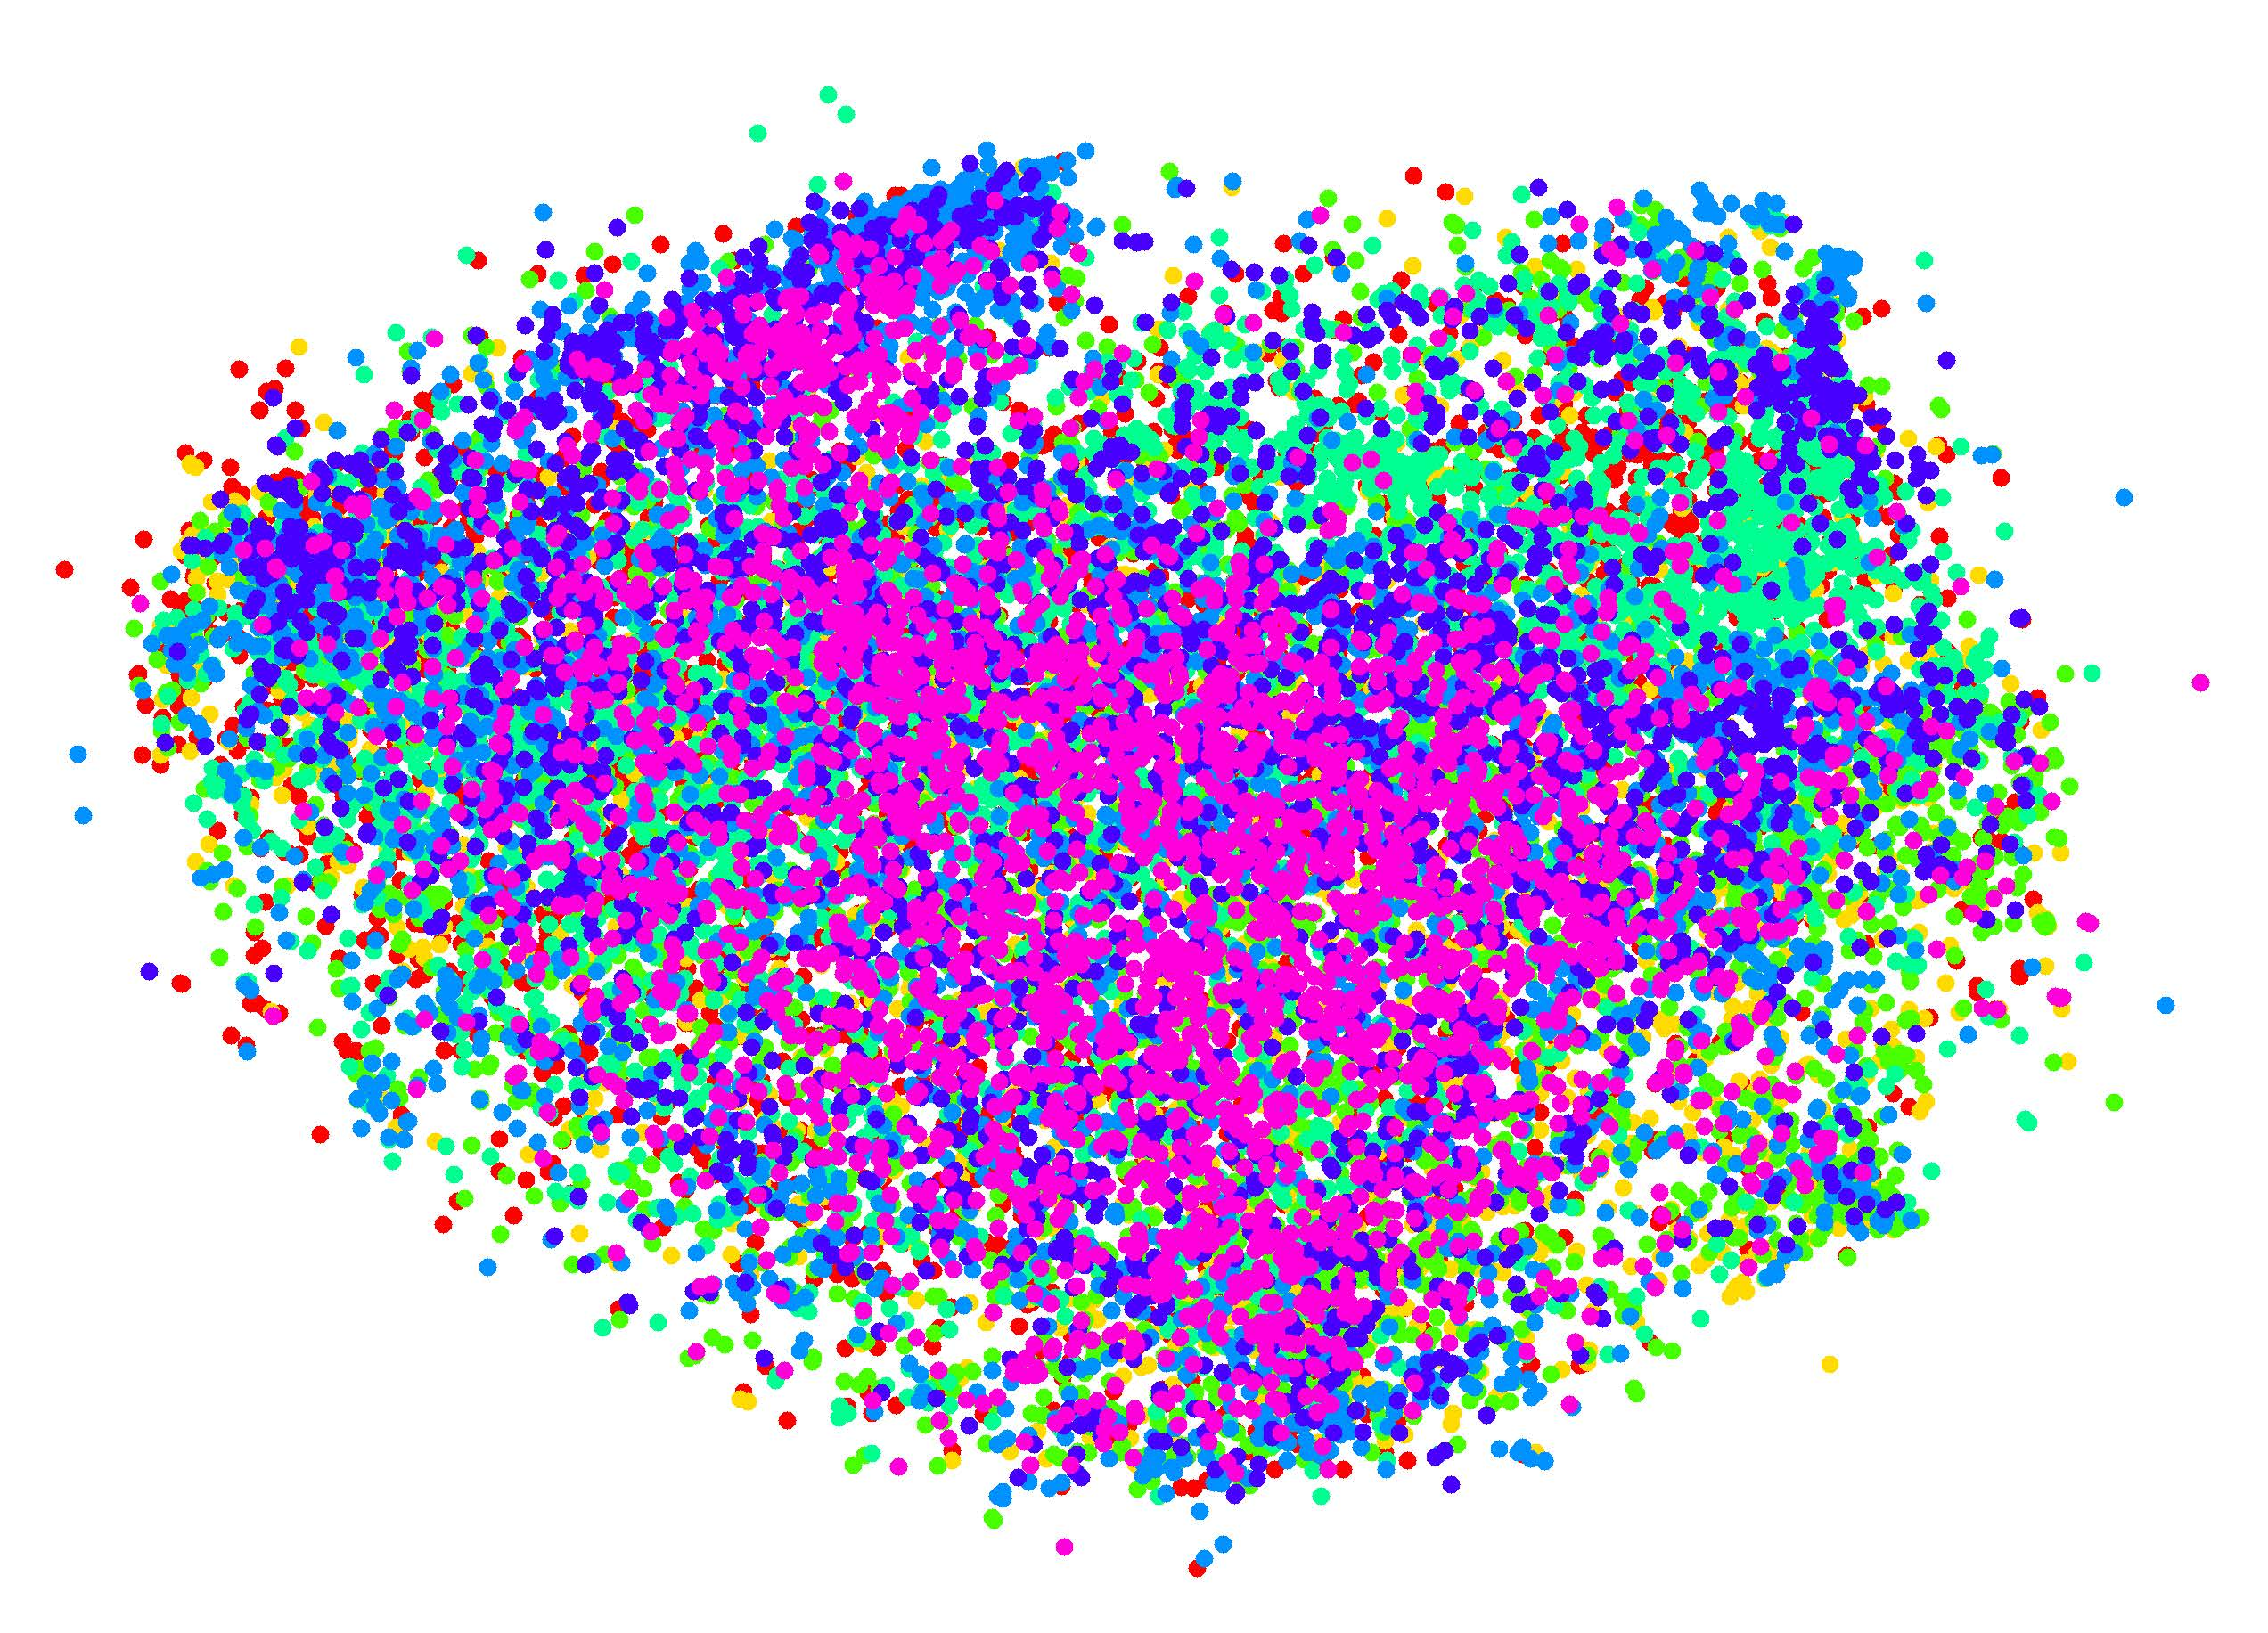
\includegraphics[width=0.5\textwidth]{figures/DECAF1}
\caption{训练损失收敛曲线}
\label{fig:convergence}
\end{figure}

\section{消融实验}
\esection{Ablation Study}
\label{sec:ablation}

表\ref{tab:ablation}的消融实验表明，各个模块对最终性能均有显著贡献。

\begin{table}[htbp]
\centering
\caption{消融实验结果}
\label{tab:ablation}
\begin{tabular}{lccc}
\toprule
配置 & 准确率 (\%) & F1 分数 \\
\midrule
仅基线 & 82.15 & 0.803 \\
去掉模块 A & 79.32 & 0.781 \\
去掉模块 B & 71.88 & 0.702 \\
完整模型 & \textbf{91.27} & \textbf{0.905} \\
\bottomrule
\end{tabular}
\end{table}
